\documentclass[10pt, a4paper]{amsart}
%\usepackage[english,norsk]{babel}
\usepackage[english]{babel}
\usepackage[utf8]{inputenc}

\usepackage{geometry}   % Margins
\usepackage{graphicx}   % Images
\usepackage{float}      % Image floating
\usepackage{siunitx}    % SI-units
\usepackage{amsmath}
\newcommand{\bs}[1]{\boldsymbol{#1}} % abbreviation of boldsymbol
\usepackage{algorithm}
\usepackage{verbatim}
\usepackage{url}
\usepackage{hyperref}
\usepackage{listings}
\usepackage{framed}
\numberwithin{figure}{section}
\numberwithin{table}{section}
\bibliographystyle{plain}

\usepackage{color}
%\usepackage{multicol}
%\setlength\columnsep{14pt}

\definecolor{codegreen}{RGB}{0, 146, 146}
\definecolor{codegray}{rgb}{0.4,0.4,0.4}
\definecolor{codeblue}{RGB}{0, 109, 219}
\definecolor{backcolour}{rgb}{0.9,0.9,0.9}

\lstdefinestyle{mystyle}{
    backgroundcolor=\color{backcolour},
    commentstyle=\color{codegreen},
    keywordstyle=\color{magenta},
    numberstyle=\tiny\color{codegray},
    stringstyle=\color{codeblue},
    basicstyle=\footnotesize,
    breakatwhitespace=false,
    showstringspaces=false,
    breaklines=true,
    captionpos=b,
    keepspaces=true,
    numbers=left,
    numbersep=5pt,
    showspaces=false,
    basicstyle=\footnotesize \ttfamily \color{black} \bfseries,
    xleftmargin=0.4cm,
    frame=tlbr, framesep=0.1cm, framerule=0pt,
    showtabs=false,
    tabsize=2
}

\lstset{style=mystyle}


\title[Mandatory exercise 3]{IN5270 \\ \large
Mandatory eercise 3}
\author[Husom]{Erik Johannes B. L. G. Husom \\ \\ \today}


\begin{document}



\maketitle


\tableofcontents

%\begin{multicols}{2}

\section{Description of the problem}


The goal is to compute deflection of a cable with sine functions. We have a hanging cable
with tension, and the cable has a deflection $w(x)$ which is governed by:

\begin{equation}
    Tw''(x) = l(x),
\end{equation}
where the variables are:

- $L$: Length of cable
- $T$: Tension on cable
- $w(x)$: Deflection of cable
- $l(x)$: Vertical load per unit length

Cable is fixed at $x = 0$ and $x = L$, and the boundary conditions are $w(0) = w(L) = 0$. Deflection 
is positive upwards and $l$ is positive when it acts downwards.

Assuming $l(x) = \text{const}$, the solution is symmetric around $x = L/2$. For a
function $w(x)$ that is symmetric around a point $x_0$, we have that

\begin{equation}
w(x_0 - h) = w(x_0 + h),
\end{equation}

which means that

\begin{equation}
(3) lim_{h->0} (w(x_0+h) - w(x_0 - h))/(2h) = 0.
\end{equation}

We can therefore halve the domain, since it is symmetric. That limits the
problem to find $w(x)$ in $[0, L/2]$, with boundary conditions $w(0) = 0$
and $w'(L/2) = 0$.

Scaling of variables:

\begin{align}
    \overline{x} &= x/(L/2)  \hspace{0.5cm}    \text{(setting $x =
    \overline{x}$ in code for easier notation)}\\
    u &= w/w_c \hspace{0.5cm} \text{(where $w_c$ is a characteristic size of $w$)}
\end{align}

By putting this into the original equation we get

\begin{equation}
    \frac{4T w_c}{L^2} u''(\overline{x}) = l = \text{const}. 
\end{equation}

    We set $|u''(\overline{x})|= 1$, and we get $w_c = 0.25lL^2/T$, and the scaled problem is

    \begin{equation}
        u'' = 1, \overline{x} \in (0,1), u(0) = 0, u'(1) = 0.
    \end{equation}


\section{Exact solution of $u$}

The exact solution of $u$ is easily found by integrating two times, and using
the boudnary conditions to find the unknown constants:

\begin{align}
    u'' &= 1,\\
    u' &= x + C,\\
    u'(1) &= 0 \Rightarrow C = -1,\\
    u &= \frac{1}{2}x^2 -x + D,\\
    u(0) &= 0 \Rightarrow D = 0,\\
    u &= \frac{1}{2}x^2 - x.
\end{align}

\section{Using two P1 elements to approximate the function}

In our case, with two elements, we will have three nodes. The basis function of
the three nodes are easily found by using Lagrange polynomials, which is
calculated within each element $\Omega_i$ that the basis function is defined in
(since we only have two elements in this case, the middle basis function
$\varphi_1$ is defined in both elements, while the other two basis functions
are defined in only one element). We have a constant distance between each
node $h = 0.5$, and our nodes is $x_0 = 0, x_1 = 0.5, x_2 = 1$. Then we get:

\[
    \varphi_0 =
    \begin{cases}
        \frac{x - x_{i+1}}{x_i - x_{i+1}} = \frac{x - x_1}{-h} = -2x + 1 & x_0 \leq x
        < x_1 \\
    \end{cases}
\]
\[
    \varphi_1 =
    \begin{cases}
        \frac{x - x_{i-1}}{x_i - x_{i-1}} = \frac{x - x_0}{h} = 2x & x_0 \leq x
        < x_1 \\
        \frac{x - x_{i+1}}{x_i - x_{i+1}} = \frac{x - x_2}{-h} = -2x + 2 & x_1
        \leq x < x_2 \\
    \end{cases}
\]
\[
    \varphi_2 =
    \begin{cases}
        \frac{x - x_{i-1}}{x_i - x_{i-1}} = \frac{x - x_1}{h} = 2x - 1 & x_1
        \leq x < x_2 \\
    \end{cases}
\]

Our problem expressed in its Galerking formulation is:

\begin{equation}
    (u'', v) = (f, v),
\end{equation}

where $f=1$. We use integration by parts to reduce the order of the derivative
of u:

\begin{align}
    \int_0^L u''(x)v(x) dx &= -\int_0^L u'(x) v'(x) dx + [vu']_0^L,\\
    &= -\int_0^L u'(x) v'(x) dx + u'(L)v(L) - u'(0)v(0).
\end{align}

We have that $u'(L) = 0$, so the middle term vanishes. Since $u(0)=0$, we must
also require $v(0)=0$. Our variational formulation becomes

\begin{align}
    - (u', v') &= (1, v),\\
    (u', v') &= - (1, v).
\end{align}


We can then find the element matrix for $\Omega_0$ ($\varphi^0_1$ means
$\varphi_1$ as defined in $\Omega_o$), by the formula:

\begin{equation}
    A_{i,j} = \int_0^{0.5} \varphi'_i \varphi'_j dx,
\end{equation}

and the $b$-vector by the formula

\begin{equation}
    b_i = - \int_0^{0.5} \varphi_i dx.
\end{equation}

We get:

\begin{gather*}
A^{(0)}=
\begin{pmatrix}
\int^{0.5}_{0}\varphi'_0\varphi'_0 dx & \int^{0.5}_{0}\varphi'^0_1\varphi'_0dx\\
    \int^{0.5}_{0}\varphi'_0\varphi'^0_1dx &
    \int^{0.5}_{0}\varphi'^0_1\varphi'^0_1 dx
\end{pmatrix}=
\begin{pmatrix}
2 & -2\\
-2 & 2
\end{pmatrix}
\end{gather*}

By using the formula for the element vector $b$, we obtain

\begin{gather*}
    b^{(0)} = 
    \begin{pmatrix}
        [-x^2 + x]_0^{0.5} \\
        [x^2]_0^{0.5} 
    \end{pmatrix} =
    \begin{pmatrix}
        -0.25\\
        -0.25
    \end{pmatrix}
\end{gather*}


We do the similar thing for element $\Omega_1$:

\begin{gather*}
A^{(1)}=
\begin{pmatrix}
2 & -2\\
-2 & 2
\end{pmatrix}
\end{gather*}

\begin{gather*}
    b^{(1)} = 
    \begin{pmatrix}
        [-x^2 + 2x]_{0.5}^{1} \\
        [x^2 - x]_{0.5}^{1} 
    \end{pmatrix} =
    \begin{pmatrix}
        -0.25\\
        -0.25
    \end{pmatrix}
\end{gather*}

We gather the element matrices and element vectors:

\begin{gather*}
A=
\begin{pmatrix}
2 & -2 &0\\
-2 & 4 & -2\\
0& -2 &2
\end{pmatrix}, \qquad
b=
\begin{pmatrix}
-0.25 \\
-0.5\\
-0.25
\end{pmatrix}
\end{gather*}

This will now be used to solve the linear system $Ac = b$. We have a boundary
condition $u(0) = 0$, which means that we must modify the linear system with
$c_0 = 0$, and therefore we set $b_0 = 0$ and the first row of A to 0 (except
the first element, which is set to 1). This way, we ensure that $u(0)=0$. The
result is shown in figure \ref{fig:cable_2P1}. My code is in the file
\texttt{cable\_2P1.py}, which is included in the same GitHub repository as this
report. To solve the linear system, I have used the \texttt{numpy.linalg.solve}
function.

\begin{figure}
       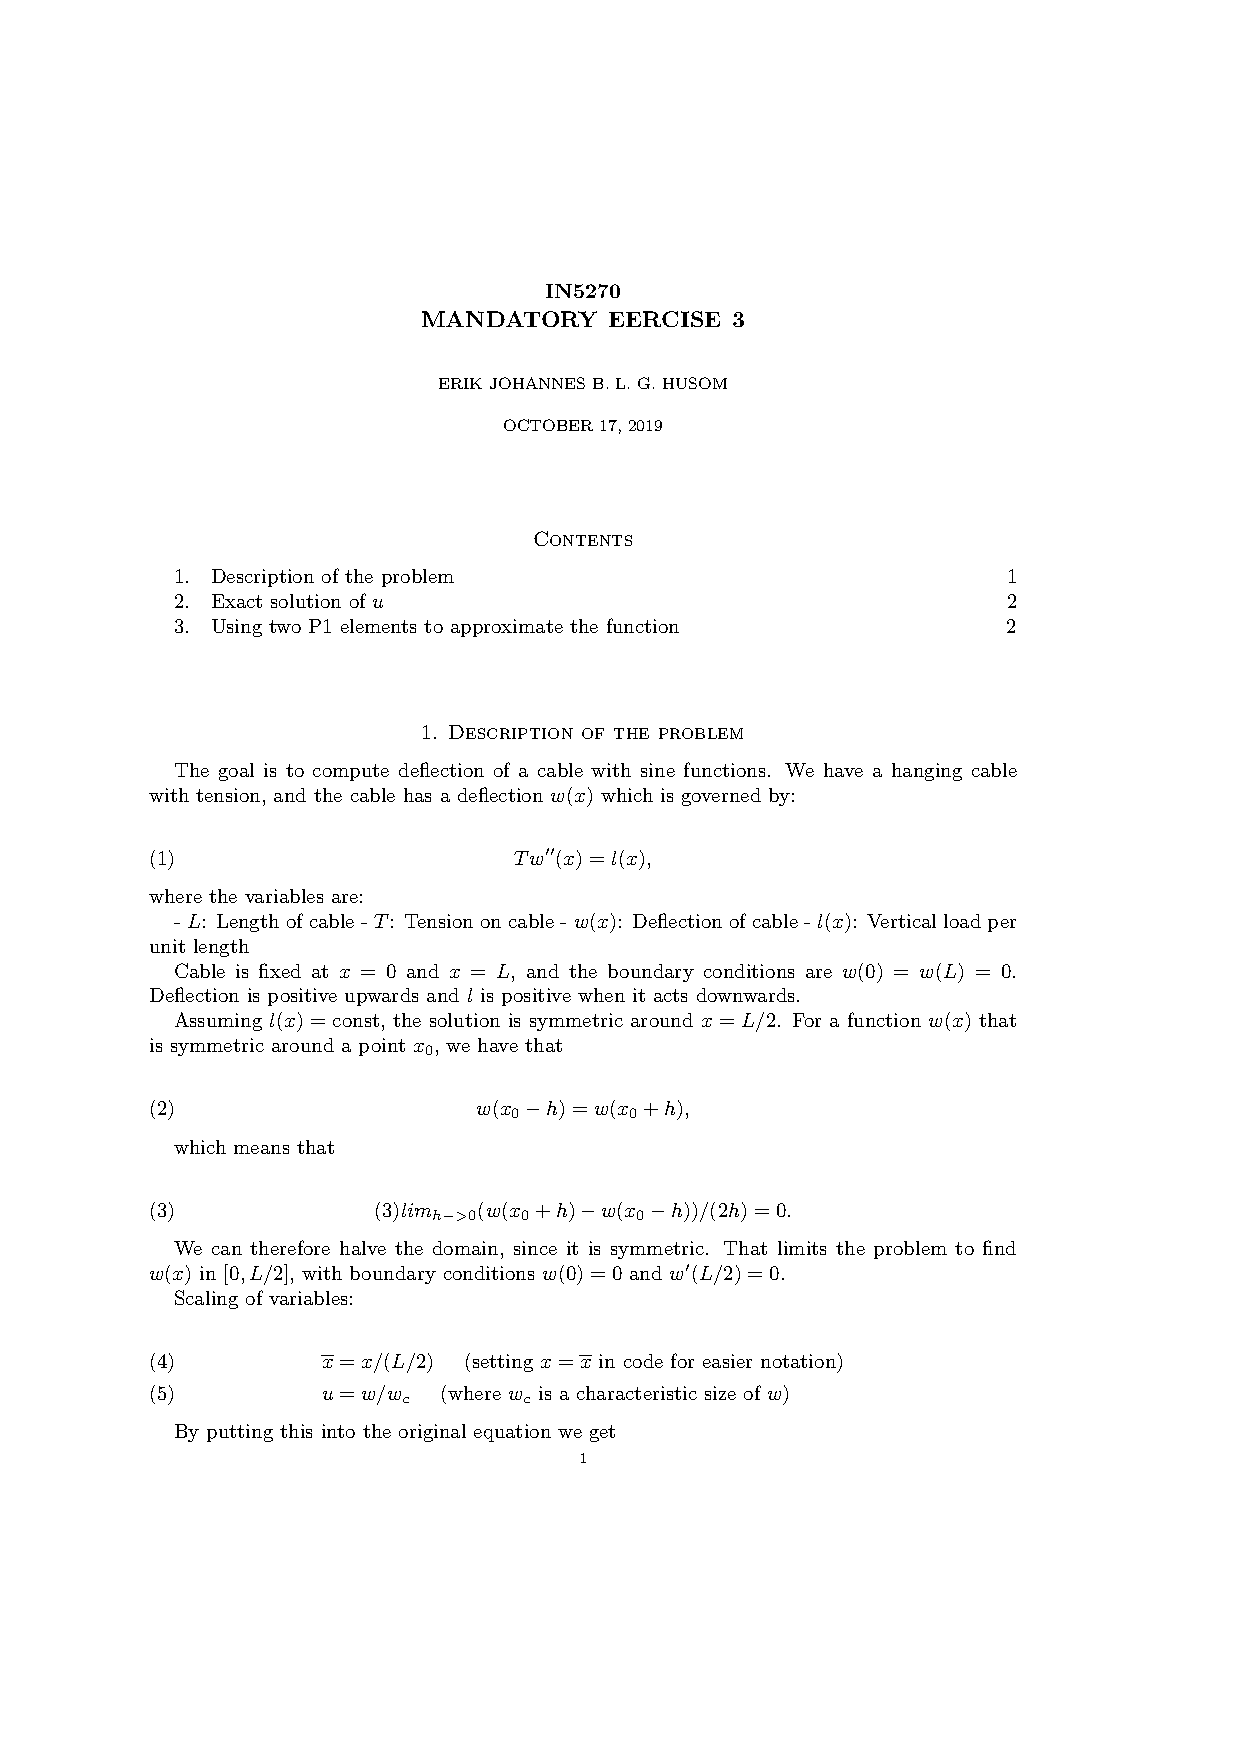
\includegraphics[width=\linewidth]{cable_2P1.png}
       \caption{Approximating $u_e$ by using P1 elements.}
       \label{fig:cable_2P1}
\end{figure}

%\end{multicols}
\end{document}

